%%%%%%%%%%%%%%%%%%%%%%%%%%%%%%%%% LAB-5 %%%%%%%%%%%%%%%%%%%%%%%%%%%%%%%%%%
%>>>>>>>>>>>>>>>>>>>>>>>>>> ПЕРЕМЕННЫЕ >>>>>>>>>>>>>>>>>>>>>>>>>>>>>>>>>>>
%>>>>> Информация о кафедре
%\newcommand{\year}{2021 г.}  % Год устанавливается автоматически
\newcommand{\city}{Санкт-Петербург}  %  Футер, нижний колонтитул на титульном листе
\newcommand{\university}{Национальный исследовательский университет ИТМО}  % первая строка
\newcommand{\department}{Факультет программной инженерии и компьютерной техники}  % Вторая строка
\newcommand{\major}{Направление программной инженерии}  % Треьтя строка
%<<<<< Информация о кафедре

%>>>>> Назание работы
\newcommand{\reporttype}{ОТЧЕТ ПО ДОМАШНЕЙ РАБОТЕ} % тип работы, (главный заголовок титульного листа)
\newcommand{\lab}{Домашняя работа}          % вид работы
\newcommand{\labnumber}{}                    % порядковый номер работы
\newcommand{\subject}{Компьютерные сети}         % учебный предмет
\newcommand{\labtheme}{Методы кодирования в компьютерных сетях}            % Тема лабораторной работы

\newcommand{\student}{Тюрин Иван Николаевич}    % определение ФИО студента
\newcommand{\studygroup}{P33102}                 % определение учебной группы 
\newcommand{\teacher}{% принимающий
    Авксентьева Е. Ю.,\\[1mm]% ФИО лектора
     Алиев Т. И.% ФИО практика
}
%<<<<<<<<<<<<<<<<<<<<<<<<<< ПЕРЕМЕННЫЕ <<<<<<<<<<<<<<<<<<<<<<<<<<<<<<<<<<<


%>>>>>>>>>>>>>>>>>>>>>> ПРЕАМБУЛА >>>>>>>>>>>>>>>>>>>>>>>>>

%>>>>>>>>>>>>>>>>>> ПРЕАМБУЛА >>>>>>>>>>>>>>>>>>>>
\documentclass[14pt,final,oneside]{extreport}% класс документа, характеристики
%>>>>> Разметка документа
\usepackage[a4paper, mag=1000, left=3cm, right=1.5cm, top=2cm, bottom=2cm, headsep=0.7cm, footskip=1cm]{geometry} % По ГОСТу: left>=3cm, right=1cm, top=2cm, bottom=2cm,
\linespread{1} % межстройчный интервал по ГОСТу := 1.5
%<<<<< Разметка документа

%>>>>> babel c языковым пакетом НЕ должны быть первым импортируемым пакетом
\usepackage[utf8]{inputenc}
\usepackage[T1,T2A]{fontenc}
\usepackage[russian]{babel}
%<<<<<

%\usepackage{cmap} %поиск в pdf

%>>>...>> прочие полезные пакеты
\usepackage{amsmath,amsthm,amssymb}
\usepackage{mathtext}
\usepackage{indentfirst}
\usepackage{graphicx}
\usepackage{float}
\graphicspath{{/home/ivan/itmo/informatics/latex}}
\DeclareGraphicsExtensions{.pdf,.png,.jpg}
%\usepackage{bookmark}

\usepackage[dvipsnames]{xcolor}
\usepackage{hyperref}  % Использование ссылок
\hypersetup{%  % Настройка разметки ссылок
    colorlinks=true,
    linkcolor=blue,
    filecolor=magenta,      
    urlcolor=magenta,
    %pdftitle={Overleaf Example},
    %pdfpagemode=FullScreen,
}

\usepackage{diagbox}
\usepackage[letterspace=150]{microtype} % Спэйсинг (межбуквенный интервал для саголовка) \lsstyle
% \usepackage{csvsimple} %импорт содержимого таблицы из csv

%>>> верстка в 2 колонки
\usepackage{multicol} % многоколоночная верстка
\setlength{\columnsep}{.15\textwidth} % определение ширины разделителя между колонками

\usepackage{tikz} % пакет для векторной графики, чтобы рисовать красивый разделитель колонок
% %> кастомный разделитель колонок
% \usetikzlibrary{arrows.meta,decorations.pathmorphing,backgrounds,positioning,fit,petri}
% \usepackage{multicolrule} % Для кастомизации разделителя колонок
% \SetMCRule{                     % кастомизация разделителя колонок multicolrule
%     width=2pt,
%     custom-line={               % Tikz код для кастомизации линии разделителя
%         \draw [                 % Рисовать
%             decorate,           % декорированную (требуются спец настройки пакетов tikz (см. импорт выше)
%             decoration={        % вид декорирования
%                 snake, % Тип - змейка (волнистая)
%                 amplitude=.5mm, % ширина волн
%                 pre length=0mm, % участок прямой линии от начала
%                 %segment length=0mm, % учасок волнистой линии
%                 post length=0mm % участок прямой линии от конца
%             },
%             line width=1pt,
%             step=10pt
%         ] 
%         (TOP) to (BOT); % сверху и до низа колонки
%     }, 
%     extend-top=-5pt, % Вылезти за верхнюю границу колонки 
%     extend-bot=-7pt % Вылезти за нижнюю границу колонки  
% }
%% < кастомный разделитель колонок
%%<<< верстка в 2 колонки

%>>>>> Использование листингов
\usepackage{listings} 
\usepackage{caption}
\DeclareCaptionFont{white}{\color{white}} 
\DeclareCaptionFormat{listing}{\colorbox{gray}{\parbox{\textwidth}{#1#2#3}}}

\captionsetup[lstlisting]{format=listing,labelfont=white,textfont=white} % Настройка вида описаний
\lstset{  % Настройки вида листинга
inputencoding=utf8, extendedchars=\true, keepspaces = true, % поддержка кириллицы и пробелов в комментариях
language={},            % выбор языка для подсветки (здесь это Pascal)
basicstyle=\small\sffamily, % размер и начертание шрифта для подсветки кода
numbers=left,               % где поставить нумерацию строк (слева\справа)
numberstyle=\tiny,          % размер шрифта для номеров строк
stepnumber=1,               % размер шага между двумя номерами строк
numbersep=5pt,              % как далеко отстоят номера строк от подсвечиваемого кода
backgroundcolor=\color{white}, % цвет фона подсветки - используем \usepackage{color}
showspaces=false,           % показывать или нет пробелы специальными отступами
showstringspaces=false,     % показывать илигнет пробелы в строках
showtabs=false,             % показывать или нет табуляцию в строках
frame=single,               % рисовать рамку вокруг кода
tabsize=2,                  % размер табуляции по умолчанию равен 2 пробелам
captionpos=t,               % позиция заголовка вверху [t] или внизу [b] 
breaklines=true,            % автоматически переносить строки (да\нет)
breakatwhitespace=false,    % переносить строки только если есть пробел
escapeinside={\%*}{*)}      % если нужно добавить комментарии в коде
}

\definecolor{codegreen}{rgb}{0,0.6,0}
\definecolor{codegray}{rgb}{0.5,0.5,0.5}
\definecolor{codepurple}{rgb}{0.58,0,0.82}
\definecolor{backcolour}{rgb}{0.95,0.95,0.92}

\lstdefinestyle{mystyle}{
    backgroundcolor=\color{backcolour},   
    commentstyle=\color{codegreen},
    keywordstyle=\color{magenta},
    numberstyle=\tiny\color{codegray},
    stringstyle=\color{codepurple},
    basicstyle=\ttfamily\footnotesize,
    breakatwhitespace=false,         
    breaklines=true,                 
    captionpos=b,                    
    keepspaces=true,                 
    numbers=left,                    
    numbersep=5pt,                  
    showspaces=false,                
    showstringspaces=false,
    showtabs=false,                  
    tabsize=2
}
\lstset{style=mystyle}
%<<<<< Использование листингов


\sloppy % Решение проблем с переносами (с. 119 книга Львовского)
\emergencystretch=25pt


%>>>>>>>>>>>>>>>> ДОПОЛНИТЕЛЬНЫЕ КОМАНДЫ {Для соответствия ГОСТ} >>>>>>>>>>>>>>
%>>>>>> математические функции для удобства
\newcommand{\tx}{\text}
\newcommand{\eps}{\varepsilon}
\renewcommand{\phi}{\varphi}
\newcommand{\limit}{\displaystyle\lim}
\newcommand{\oo}{\infty}
\newcommand{\De}{\Delta}
\newcommand{\cd}{\cdot}
\newcommand{\df}{\partial}
\newcommand{\ndash}{\textendash}
\newcommand{\mdash}{\textemdash}

%>>>>> Аннотирование
\newcommand{\note}[2]{\overbrace{#1}^{#2}}% скобка сверху для комментария
% \overset{}{}% для указания символа над другим смиволом
% \underset{}{}% для указания символа под другим смиволом
%<<<<< Аннотирование

%>>>>>> Матрицы
\DeclareMathOperator{\rank}{rank}
\newcommand{\tvec}[1]{\mathbfit{#1}}% "text vector"
\newcommand{\mtx}[1]{\mathrm{#1}}
\newcommand{\transposed}[1]{{#1}^{\mathrm{T}}}
%>>>>>> Матрицы

%>>>>> Скобки
\newcommand{\lt}{\left}
\newcommand{\rt}{\right}
\newcommand{\la}{\langle}% '<'
\newcommand{\ra}{\rangle}% '>'
\newcommand{\avg}[1]{\langle{#1}\rangle}% '<X>'
%<<<<< Скобки

%>>>>> Дроби
\newcommand{\cf}[2]{\cfrac{#1}{#2}}
\newcommand{\fr}[2]{\frac{#1}{#2}}
%<<<<< Дроби


%>>>>> Стрелки
\newcommand{\Rarr}{\Rightarrow}% ⇒ следствие | лучше использовать \implies
\newcommand{\LRarr}{\Leftrightarrow}% равносильно | лучше  использовать \iff
\newcommand{\rarr}{\xrightarrow{}}% → стрелка вправо
\newcommand{\nwarr}{\nwarrow}% ↖ север-запад стрелка
\newcommand{\nearr}{\nearrow}% ↗ север-восток стрелка
\newcommand{\swarr}{\swarrow}% ↙ юг-запад стрелка
\newcommand{\searr}{\searrow}% ↘ юг-восток стрелка

\newcommand{\raises}{\nwarrow}% возрастает
\newcommand{\increases}{\nwarrow}% возрастает
\newcommand{\falls}{\swarrow}% убывает
\newcommand{\decreases}{\swarrow}% убывает

%{{{
\makeatletter
\newcommand{\impliesby}[2][]{\ext@arrow 0359\Leftrightarrowfill@{#1}{#2}}% следствие с надписью
\makeatother
%}}}

%{{{
\makeatletter
\newcommand{\iffby}[2][]{\ext@arrow 0359\Rightarrowfill@{#1}{#2}}% равносильность с надписью
\makeatother
%}}}
%<<<<< Стрелки

% Функции для удобного описания формул: https://tex.stackexchange.com/questions/95838/how-to-write-a-perfect-equation-parameters-description



%<<<<<< математические функции для удобства
%>>>>>> Стиль текста
\newcommand{\hex}[1]{\texttt{0{\footnotesize{x}}#1}}
\newcommand{\ttt}[1]{\texttt{#1}}
%<<<<<< Стиль текста

\newcommand\Chapter[3]{%
    % Принимает 3 аргумента - название главы и дополнительный заголовок и множитель ширины загловка (можно ничего)
    \refstepcounter{chapter}%
    \chapter*{%
        %\hfill % заполнение отступом пространства до заголовка
        \begin{minipage}{#3\textwidth} % Можно изменить ширину министраницы (заголовка)
            \flushleft % Выранивание заголовка по левому краю параграфа (заголовка)
            %\flushright % Выранивание заголовка по правому краю параграфа (заголовка)
            \begin{huge}%
                % Отключена нумерация глав в тексте:
                % \textbf{\chaptername\ \arabic{chapter}\\}
                \textbf{#1}% Первый заголовок
            \end{huge}%
            \\% Перенос сторки
            \begin{Huge}
                #2% Второй заголовок
            \end{Huge}
        \end{minipage}
    }%
    % Отключена нумерация для chapter в toc (table of contents), т.е. Оглавлении (Содержании):
    % \addcontentsline{toc}{chapter}{\arabic{chapter}. #1}
    % Представление главы в содержании:
    \addcontentsline{toc}{chapter}{#1. #2}%
}

\newcommand\Section[1]{
    % Принимает 1 аргумент - название секции
    \refstepcounter{section}
    \section*{%
        \raggedright
        % Отключена дополнительная нумерация chapter в section в тексте документа:
        % \arabic{chapter}.\arabic{section}. #1}
        % Отключена любая нумарация section в тексте документа: 
        \arabic{section}. #1%
    }
    
    % Отключена дополнительная нумерация chapter в section в toc (table of contents) Оглавлении (Содержании):
    % \addcontentsline{toc}{section}{\arabic{chapter}.\arabic{section}. #1}
    \addcontentsline{toc}{section}{\arabic{section}. #1} 
}


\newcommand\Subsection[1]{
    % Принимает 1 аргумент - название подсекции
    \refstepcounter{subsection}
    \subsection*{%
        \raggedright%
        % Отключена дополнительная нумерация chapter в section в тексте документа (можно добавить отступ с помощью \hspace*{12pt}):
        % \arabic{chapter}.\arabic{section}.\arabic{subsection}. #1}
        \arabic{section}. \arabic{subsection}. #1
    }
    % Отключена дополнительная нумерация chapter в section в Оглавлении (Содержании):
    %\addcontentsline{toc}{subsection}{\arabic{chapter}.\arabic{section}.\arabic{subsection}. #1}
    \addcontentsline{toc}{subsection}{\arabic{subsection}. #1}
}


\newcommand\Figure[4]{
    % Принимает 4 аргумента - название файла изображения, ее размер в тексте, описание, лэйбл (псевдоним в формате "fig:name") 
    %
    \refstepcounter{figure}
    \begin{figure}[H] %- \usepackage {float} %[h]
        \begin{center}
            \fbox{
                \includegraphics[width=#2]{#1}
            }
        \end{center}
        \begin{center}
            Рис.~\arabic{figure}. #3.
        \end{center}
        %\caption{#3}
        \label{fig:#4}
    \end{figure}
}


\newcommand\Table[3]{
    % Принимает 3 аргумента --- лэйбл name(#1) (псевдоним в формате "tab:name"), ее описание(#2), содержание таблицы(#3)
    % ВАЖНО!: от этого способа страдает нумерация описаний, можно использовать создание таблиц через googlesheet
    %
    \renewcommand{\arraystretch}{1.2} % Установка высоты строки таблицы по умолчанию, увеличенное на 0.2 пункта
    % \refstepcounter{table}% увеличение счетчика таблиц
    \begin{table}[Htpb]% "right Here", "top", "new page", "bottom"
        \label{tab:#1}% лэйбл таблицы, для ссылок
        \resizebox{\columnwidth}{!}{% сжимает очень широкие таблицы, чтобы вместить на страницу
             #3% Содержимое таблицы
        }
        % 
        \caption{#2}% Описание стандартными средствами для используемого окружения (table)
        % \captionof{table}{#2}% Описание стандартными средствами
        % \captionof*{figure}{\flushleft \textsc\textbf{Рис. 1.}}% Описание стандартными средствами, как рисунка
        %
        %%> кастомное описание
        % \begin{flushleft}% Кастомное описание
        %     % \textsf{%
        %         \textbf{%
        %             \\[2mm]
        %             #2% Описание к картинке
        %         }%
        %         % \\[8mm]% Отступ
        %     % }%
        % \end{flushleft}
        %%< кастомное описание
    \end{table}
    \renewcommand{\arraystretch}{1} % возврат установка высоты строки таблицы по умолчанию на 1
}


\newcommand\CustomFigure[4]{ % multicols не умеют в table и figure, поэтому приходится извращаться % вставка таблицы с меткой рисунка
    % Принимает 4 аргумента - название файла изображения, ее размер в тексте, описание, лэйбл (псевдоним в формате "fig:name") 
    %
    \refstepcounter{figure}
    \begin{figure}[ht]% "here", "top"
        \begin{center}
            \includegraphics[width=#2]{#1}
        \end{center}
        %
        %\caption{#3}
        \captionof{figure}{#3}% описание стандартными средствами
        % \begin{center}
        \begin{flushleft} % Кастомное описание
            \textbf{%
                #3% Текст описания
            }
        \end{flushleft}
        % \end{center}
        %
        \label{fig:#4}% Лэйбл, для ссылок
    \end{figure}
}


\newcommand\CustomTableFigure[3]{% multicols не умеют в table и figure, поэтому приходится извращаться % вставка таблицы с меткой рисунка
    %
    % Принимает 3 аргумента --- лэйбл name(#1) (псевдоним в формате "tab:name"), ее описание(#2), содержание таблицы(#3) 
    %
    \begin{center}
        \refstepcounter{figure}
        \label{tab:#1}% лэйбл таблицы, для ссылок
        \resizebox{\columnwidth}{!}{% сжимает очень широкие таблицы, чтобы вместить на страницу
            #3% Содержание таблицы
        }
        % 
        \captionof{figure}{#2}% Описание стандартными средствами
        % \captionof*{figure}{\flushleft \textsc\textbf{Рис. 1.}}% Описание стандартными средствами
        %
        \begin{flushleft}% Кастомное описание
            % \textsf{%
                \textbf{%
                    \\[2mm]
                    #2% Описание к картинке
                }%
                % \\[8mm]% Отступ
            % }%
        \end{flushleft}
    \end{center}
}


\newcommand{\InkscapeFigure}[4]{% Вставки иллюстраций из Inkscape (pdf+latex)
    %
    % Принимает 4 параметра: #1 название файла, #2 описание, #3 лейбл #4 размер
    %
    % \begin{minipage}{#4}
        \begin{figure}[htbp]
            \centering
            \def\svgwidth{#4}
            \import{./figures/}{#1.pdf_tex}
            \caption{#2}
            \label{fig:#3}
        \end{figure}
    % \end{minipage}
}


\newcommand\Equation[3]{% Кастомное оформление выражений
    %
    % Принимает 3 аргумента --- лэйбл name (#1) (псевдоним в формате "tab:name"), его описание(#2), содержание выражения (#3) 
    %
    \textbf{#2}% описание
    \begin{equation}
        #3% содержимое выражений
        \label{eq:#1}% лэйбл
    \end{equation}
}

%<<<<<<<<<<<<<<<<<<<<<<<<<<<< ДОПОЛНИТЕЛЬНЫЕ КОМАНДЫ <<<<<<<<<<<<<<<<<<<<<<<<<<

%<<<<<<<<<<<<<<<<<<<<<< ПРЕАМБУЛА <<<<<<<<<<<<<<<<<<<<<<<<<



%%%%%%%%%%%%%%%%%%% СОДЕРЖИМОЕ ОТЧЕТА %%%%%%%%%%%%%%%%%%%%%
%>>>>>>>>>>>>>>> ''''''''''''''''''''''' >>>>>>>>>>>>>>>>>>
\begin{document}


%>>>>>>>>>>>>>>>> ОПРЕДЕЛЕНИЕ НАЗВАНИЙ >>>>>>>>>>>>>>>>>>>>
% Переоформление некоторых стандартных названий
%\renewcommand{\chaptername}{Лабораторная работа}
\renewcommand{\chaptername}{\lab\ \labnumber} % переименование глав
\def\contentsname{Содержание} % переименование оглавления
%<<<<<<<<<<<<<<<< ОПРЕДЕЛЕНИЕ НАЗВАНИЙ <<<<<<<<<<<<<<<<<<<<
% \setlength{\itemsep}{0pt} % установка расстояния между строчками в списках можно использовать локально внутри списка списке
% \setlength{\parskip}{0pt} % 
% \setlength{\parsep}{0pt}  % 

%>>>>>>>>>>>>>>>>> ТИТУЛЬНАЯ СТРАНИЦА >>>>>>>>>>>>>>>>>>>>>
%>>>>>>>>>>>>>>>>>>> ТИТУЛЬНЫЙ ЛИСТ >>>>>>>>>>>>>>>>>>>>>>>
\begin{titlepage}

    % Название университета
    \begin{center}
    \textsc{%
        \university\\[5mm]
        \department\\[2mm]
        \major\\
        \education\\
        \specialization\\
    }

    \vfill
    % Название работы
    \textbf{\reporttype\ \labnumber\\[3mm]
    курса <<\subject>> \\[6mm]
    по теме: <<\labtheme>>\\[3mm]
    }
    \end{center}


\vfill
\hfill
% Информация об авторе работы и проверяющем
\begin{minipage}{.5\textwidth}
    \begin{flushright}
        
            
        Выполнил студент:\\[2mm] 
        \student\\[2mm]
        группа: \studygroup\\[5mm]

        Преподаватель:\\[2mm] 
        \teacher

    \end{flushright}
\end{minipage}

\vfill

    % Нижний колонтитул первой страницы
    \begin{center}
        \city, \the\year\,г.
    \end{center}

\end{titlepage}
%<<<<<<<<<<<<<<<<<<< ТИТУЛЬНЫЙ ЛИСТ <<<<<<<<<<<<<<<<<<<<<<<


%<<<<<<<<<<<<<<<<< ТИТУЛЬНАЯ СТРАНИЦА <<<<<<<<<<<<<<<<<<<<<


%>>>>>>>>>>>>>>>>>>>>> СОДЕРЖАНИЕ >>>>>>>>>>>>>>>>>>>>>>>>>
% Содержание
\tableofcontents
%<<<<<<<<<<<<<<<<<<<<< СОДЕРЖАНИЕ <<<<<<<<<<<<<<<<<<<<<<<<<


%%%%%%%%%%%%%%%%%%%%%%% КОД РАБОТЫ %%%%%%%%%%%%%%%%%%%%%%%%
%>>>>>>>>>>>>>>>>>>>'''''''''''''''''>>>>>>>>>>>>>>>>>>>>>
\newpage
\Chapter{\lab\ \labnumber}{\labtheme}{}

\Section{Часть 1: методы физического и логического кодирования}

\Subsection{Этап 1}

В работе необходимо использовать свои инициалы для получения 
варианта согласно таблице кодировки, таким образом мой вариант:
$$
\text{<<ТИН>>} \to \mathtt{0xD2C8CD}
$$
и в двоичном виде
$$
\mathtt{0xD2C8CD} = \mathtt{0b\,1101`0010`1100`1000`1100`1101}.
$$
Длина полученного сообщения равна 3 байта (24 бит).

\Subsection{Этап 2}

На этом этапе выполнения работы нужно произвести физическое 
кодирование с использованием манчестерского кодирования и еще 
двух на выбор. Я выбираю RZ и AMI.
%
Так же по заданию нужно принять, что пропускная способность канала
связи равна C = 100 Мбит/с. Требуемые характеристики сигнала будем считать в соответствии с приложением в конце описания задания. 
\\

\subsubsection{Кодирование способом RZ}

Результат физического кодирования способом RZ можно видеть на рисунке \ref{fig:rz-encode} временной диаграммы сигнала.
\begin{figure}[H] % 'H' -- вставить тут же (подключен модуль), обычный вариант: 'htpb'
    \centering
    {\setlength{\fboxsep}{0pt}\setlength{\fboxrule}{1pt}%
    \fbox{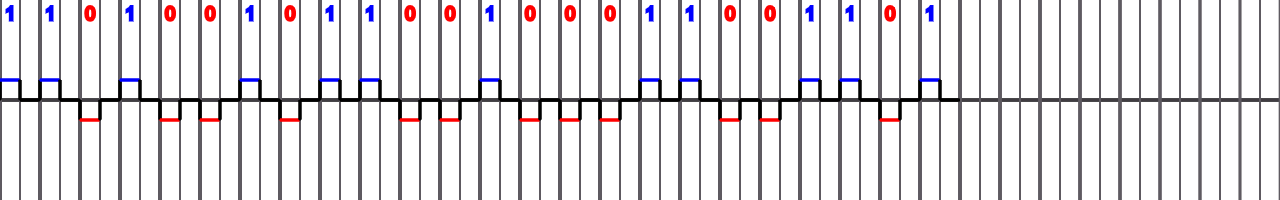
\includegraphics[width=\textwidth]{res/rz-encode.png}}}
    \caption{Результат физического кодирования способом RZ (Return-to-Zero)}
    \label{fig:rz-encode}
\end{figure}

\noindent
Характеристики сигнала рассчитанные физического сигнала изображенного на рис. \ref{fig:rz-encode} для передаваемого сообщения.
\begin{itemize}
    \item Верхняя граница частоты в передаваемом сообщении считается по самой высокочастотной составляющей сигнала, т.е. при последовательной передаче серии 1 или серии 0 период сигнала будет равен битовому интервалу (биты 1-2, 11-12, 14-16, 17-18, 19-20, 21-22 в сообщении): 
    $$
        f_\text{в} = C = 100\;\tx{МГц}.
    $$
    \item Нижняя граница в этом случае получается, если в качестве периода взять два битовых интервала:
    $$
        f_\text{н} = \cfrac{C}{2} = 50\;\tx{МГц}.
    $$
    \item Средняя частота получается средним арифметическим для всех диапазонов со всеми доступными частотами:
    $$
        f_\text{ср} = \cfrac{33\cd f_0 + 3\cd\cfrac{f_0}{2}}{36} = 95\;\tx{МГц}.
    $$
    \item Полоса пропускания для качественной передачи в соответствии со спектром $S=f_{\tx{в}}-f_{\tx{н}} = 50\;\tx{МГц}$:
    $$
        F = 100\;\tx{МГц}.
    $$    
\end{itemize}


\subsubsection{Кодирование способом AMI}

Результат физического кодирования способом AMI можно видеть на рисунке \ref{fig:ami-encode} временной диаграммы сигнала.
\begin{figure}[H] % 'H' -- вставить тут же (подключен модуль), обычный вариант: 'htpb'
    \centering
    {\setlength{\fboxsep}{0pt}\setlength{\fboxrule}{1pt}%
    \fbox{%
    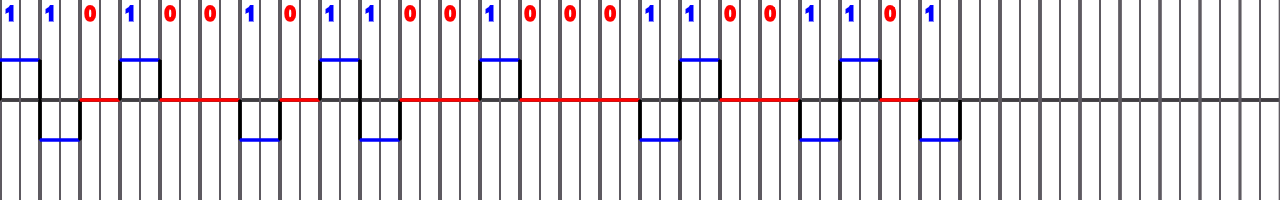
\includegraphics[width=\textwidth]{res/ami-encode.png}}}
    \caption{Результат физического кодирования способом AMI (Bipolar Alternate Mark Inversion)}
    \label{fig:ami-encode}
\end{figure}

\noindent
Характеристики сигнала:
\begin{itemize}
    \item Верхняя граница частоты в передаваемом сообщении:
    $$
        f_\text{в} = \cfrac{C}{2} = 50\;\tx{МГц},
    $$
    \item Нижняя граница теоретически нулевая, но в данном сообщении достигается, если рассмотреть передачу трёх 0 подряд (14-16 биты), период в этом случае равен 6 битовым интервалам:
    $$
        f_\text{н} = \cfrac{C}{6} = 16,67\;\tx{МГц}.
    $$
    \item Средняя частота:
    $$
        f_\text{ср} = \cfrac{15\cd f_0 + 6\cd\cfrac{f_0}{2} + 3\cd\cfrac{f_0}{3}}{24} = 39.58\;\tx{МГц}.
    $$
    \item Полоса пропускания для качественной передачи в соответствии со спектром $S=f_{\tx{в}}-f_{\tx{н}} = 33,33\;\tx{МГц}$:
    $$
        F = 100\;\tx{МГц}.
    $$    
\end{itemize}


\subsubsection{Кодирование способом Manchester-2}

Результат физического кодирования способом M2 (Manchester-2) можно видеть на рисунке \ref{fig:m2-encode} временной диаграммы сигнала.
\begin{figure}[H] % 'H' -- вставить тут же (подключен модуль), обычный вариант: 'htpb'
    \centering
    {\setlength{\fboxsep}{0pt}\setlength{\fboxrule}{1pt}%
    \fbox{%
    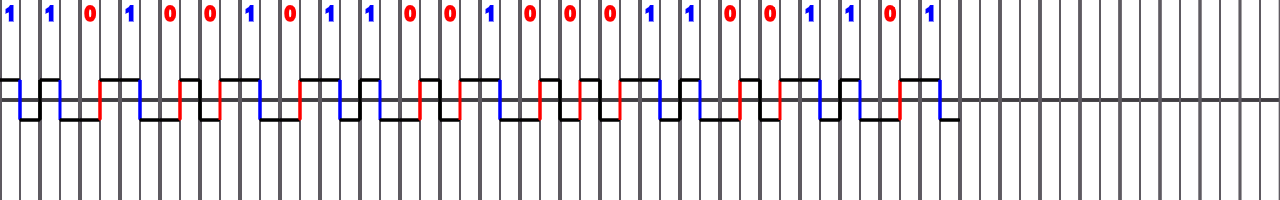
\includegraphics[width=\textwidth]{res/m2-encode.png}}}
    \caption{Результат физического кодирования способом M2 (Manchester-2)}
    \label{fig:m2-encode}
\end{figure}

\noindent
Характеристики сигнала:
\begin{itemize}
    \item Верхняя граница частоты в передаваемом сообщении:
    $$
        f_\text{в} = C = 100\;\tx{МГц},
    $$
    \item Нижняя граница достигается если рассмотреть передачу подряд различных значений: 0 и 1 или 1 и 0 (1-2, 2-3... биты), период в этом случае равен 2 битовым интервалам:
    $$
        f_\text{н} = \cfrac{C}{2} = 50\;\tx{МГц}.
    $$
    \item Средняя частота:
    $$
        f_\text{ср} = \cfrac{20\cd f_0 + 28\cd\cfrac{f_0}{2}}{48} = 70.833\;\tx{МГц}.
    $$
    \item Полоса пропускания для качественной передачи в соответствии со спектром $S=f_{\tx{в}}-f_{\tx{н}} = 50\;\tx{МГц}$:
    $$
        F = 100\;\tx{МГц}.
    $$    
\end{itemize}

Как можно видеть, все методы кодирования имеют свои преимущества и недостатки:  RZ и M2 имеют возможность самосинхронизации и лишены постоянной составляющей сигнала (минимальная частота теоретически не нулевая), но требуют больше спектр частот чем AMI.

\Subsection{Этап 3}

Сообщение закодированное при помощи 4B/5B: 
$$
\mathtt{0b\,1101`1101`0011`0101`0010`1101`0110`11}.
$$ 
16-ый код сообщения полученного при помощи 4B/5B: \verb|0x374D4B5B|.
Длина сообщения полученного при этом 3,75 байта (30 бит),
чему соответствует избыточность 0,25.

\Subsection{Этап 4}

Исходное сообщение было скремблировано с использованием предложенной формулы
$$
    B_i = A_i\oplus B_{i-3}\oplus B_{i-5}
$$ 
(см. листинг \ref{lst:scramble-given}) и с помощью собственной формулы
$$
    B_i = A_i\oplus B_{i-14}\oplus B_{i-16}
$$ 
(см. листинг \ref{lst:scramble-my}). Как оказалось, для предложенной формулы происходит не эффективное кодирование, т.к. с моей формулой в полученном сообщении меньше длина последовательности одинаковых значений (2 против 8 в предложенной). 

\lstinputlisting[language=python,caption={Скремблирование исходного сообщения с исползованием предложенной формулы},label={lst:scramble-given}]{res/scramble-given.py}

\lstinputlisting[language=python,caption={Скремблирование исходного сообщения с использованием собственной формулы},label={lst:scramble-my}]{res/scramble-my.py}

\Subsection{Этап 5}

Как можно было видеть, все методы кодирования имеют свои особенности: преимущества и недостатки. Методы физического кодирования накладывают определенные ограничения на канал связи, в то время как кодирование с избыточностью этого не требует, но увеличивает длину передаваемого сообщения. Скремблирование в свою очередь требует подбора подходящей функции, т.к. для разных сообщений они по-разному эффективны.
Хорошо выглядит идея использовать эти методы кодирования одновременно для получения преимуществ каждого из них и нивелирования их недостатков, например, скремблирования и физического кодирования AMI, чтобы увеличить среднюю частоту.

\Section{Часть 2}

Для каждого этапа 6-10 были проведены необходимые симуляции в среде NetworkFurier 2.1, по результатам которых была составлена таблица 2 представленная на рисунке \ref{fig:table-2}. Максимальные номера гармоник высчитывались для подобранных минимальных номеров. При этом, для этапа 9-10 не удалось получить удобоваримые результаты, т.к. во всех случаях при максимальном номере гармоники (255) не удалось добиться передачи сообщения без помех.

\begin{figure}
    \centering
    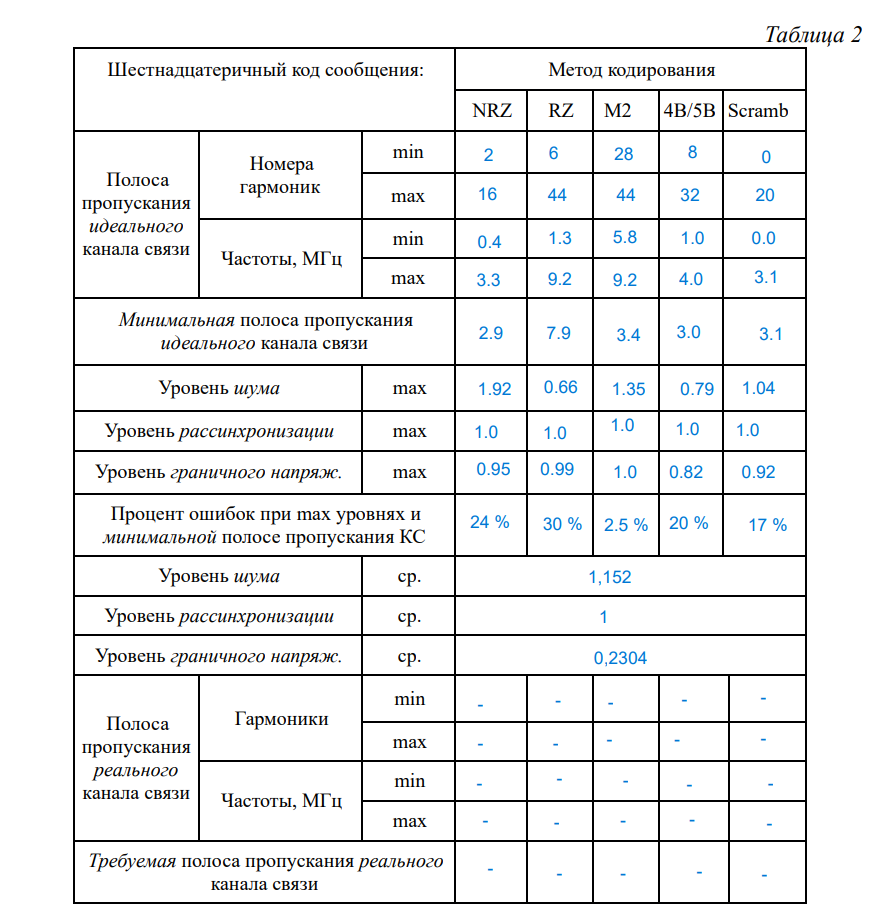
\includegraphics[width=\textwidth]{res/table-2.png}
    \caption{Результаты симуляции в среде NetworkFurier 2.1 для исходного сообщения}
    \label{fig:table-2}
\end{figure}

\Section{Вывод}

Не удалось определить какой тип кодирования лучше подходит для передачи сообщения по реальному каналу, можно сказать лишь то, что при кодировании со скремблированием (NRZ) ошибки визуально возникают реже. Теоретически манчестерский код дает лучше качество передачи при большем уровне рассинхронизации и граничного напряжения, уровень шума может быть тоже достаточно высок. Скремблирование позволяет повысить качество передачи в сравнении с обычным NRZ, но не так сильно как использование другого кодирования.  

% Прямая ссылка на интернет-ресурc: \href{https://http.cat/501}{http.cat}
\newpage
%<<<<<<<<<<<<<<<<<<<<<< КОД РАБОТЫ <<<<<<<<<<<<<<<<<<<<<<<<


%>>>>>>>>>>>>>>>> СПИСОК ЛИТЕРАТУРЫ >>>>>>>>>>>>>>>>>>>>>>>
% \include{biblist}  % Для соответсвия гост, придется доработать. Нужен файл .bib
%<<<<<<<<<<<<<<<<<<<< СПИСОК ЛИТЕРАТУРЫ <<<<<<<<<<<<<<<<<<<


\end{document}
%<<<<<<<<<<<<<<<< ,,,,,,,,,,,,,,,,,,,,,,, <<<<<<<<<<<<<<<<<
%<<<<<<<<<<<<<<<<<<< СОДЕРЖИМОЕ ОТЧЕТА <<<<<<<<<<<<<<<<<<<<
